\newpage
\section*{Задание 1: Описание и структурный анализ программного кода}
\subsection{Постановка задачи}
\noindent
Язык: Python \\
Алгоритм: Прямой проход нейронной сети (Forward Propagation) \\
Специфика кода: Матричные операции через списки списков, индексы i, j, k, магические числа, отсутствие комментариев \\
Контекст: Разбор учебного прототипа модели компьютерного зрения для встраиваемых систем\\
\newline
Необходимо:
\begin{enumerate}
	\item Сгенерировать «грязный» (нечитаемый, обфусцированный) код указанного алгоритма.
	\item Провести его анализ: определить назначение, расшифровать переменные, визуализировать логику, проверить гипотетические сценарии.
	\item Синтезировать итоговую структурированную документацию.
\end{enumerate}
\subsection{Гипотеза и системный промпт (этап 0 – генерация «грязного» кода)}
Промпт (основной модели):
\textit{«Ты – небрежный разработчик, который пишет рабочий, но максимально нечитаемый код. Реализуй на Python прямой проход (forward pass) полносвязной нейронной сети с одним скрытым слоем. Функция должна принимать входной вектор и матрицы весов. Используй только списки списков (без NumPy). Замени все осмысленные имена переменных на однобуквенные (a, b, c, i, j, k). Удали все комментарии и docstring. Используй магические числа. Сверни вычисления в сложные однострочные конструкции где возможно. Код должен быть логически верным и запускаться без ошибок.»}\\
\newpage
Ответ модели: 
\lstinputlisting[language=Python]{z1/0.py}
\noindent
\indent Анализ: Код синтаксически верен, но имена переменных не отражают сути, повсеместно используются i, j, k, магическое число 2.7182818284 (приближение e), списковые включения усложняют чтение. Отсутствуют проверки размерностей.
\subsection{Журнал диалога и итераций (работа с основной моделью)}
\noindent
\textbf{Этап 1. Первичный контекстный анализ (Zero-shot Scoping)} \\
\indent Промпт:
\textit{«Ты – Senior-разработчик, проводящий технический аудит кода. Посмотри на этот код (приведён выше). Не вдаваясь в детали реализации, определи общее назначение программы, какие входные данные она ожидает и какой результат выдаёт. Назови возможную предметную область.»}
\newpage
Ответ модели:
\begin{figure}[H]
	\centering
	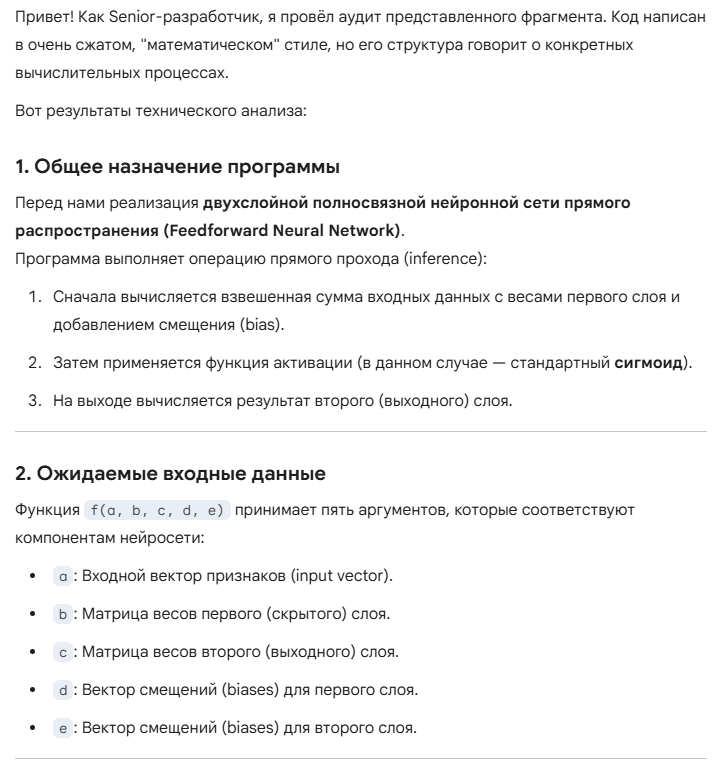
\includegraphics[width=17cm]{z1/1-1.png}
	\caption{ч.1}
\end{figure}
\newpage
\begin{figure}[H]
	\centering
	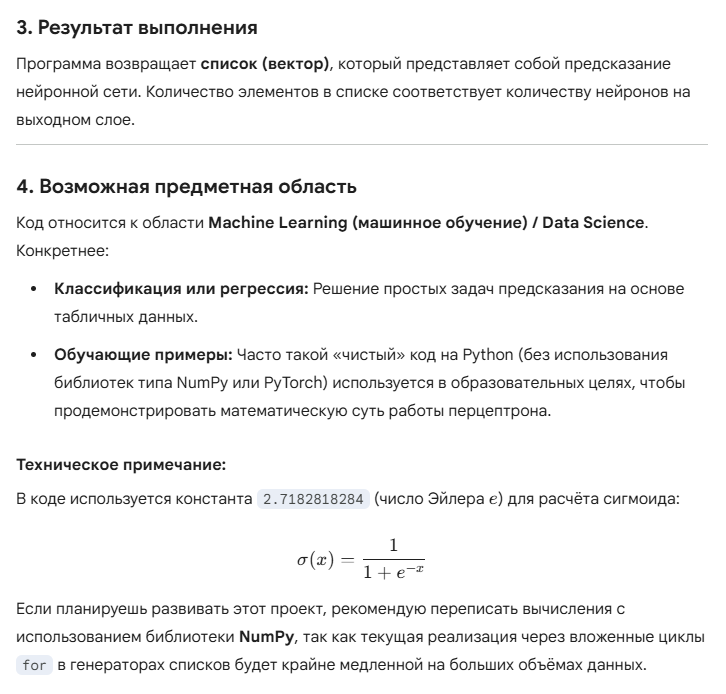
\includegraphics[width=17cm]{z1/1-2.png}
	\caption{ч.2}
\end{figure}
\noindent
\indent Анализ: Модель верно идентифицировала алгоритм, несмотря на запутанный код. Также полностю описала переменные и функцию сигмоиды. Корректировка не потребовалась.
\newpage
\noindent
\textbf{Этап 2. Глубокая интерпретация и деобфускация переменных} \\
\indent Промпт (с применением Chain of Density):
\textit{«Проведи построчный анализ. Для каждой переменной объясни её функциональную роль в контексте прямого распространения. Почему используются вложенные циклы? Что означает число 2.7182818284? Объясни логику каждого спискового включения.»}\\
\newline
Ответ модели:
\begin{figure}[H]
	\centering
	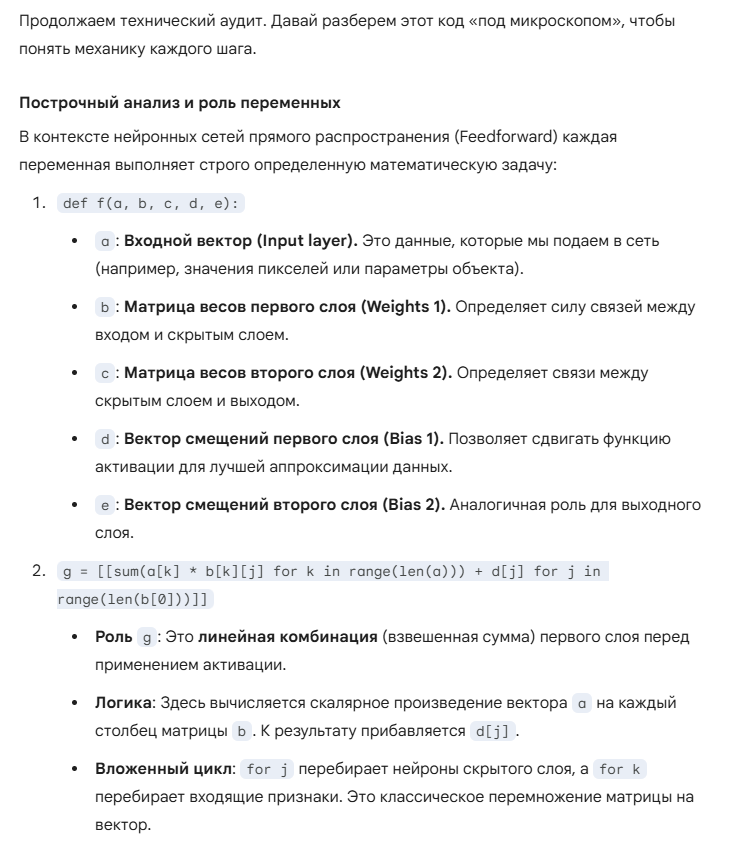
\includegraphics[width=14cm]{z1/2-1.png}
	\caption{ч.1}
\end{figure}
\newpage
\begin{figure}[H]
	\centering
	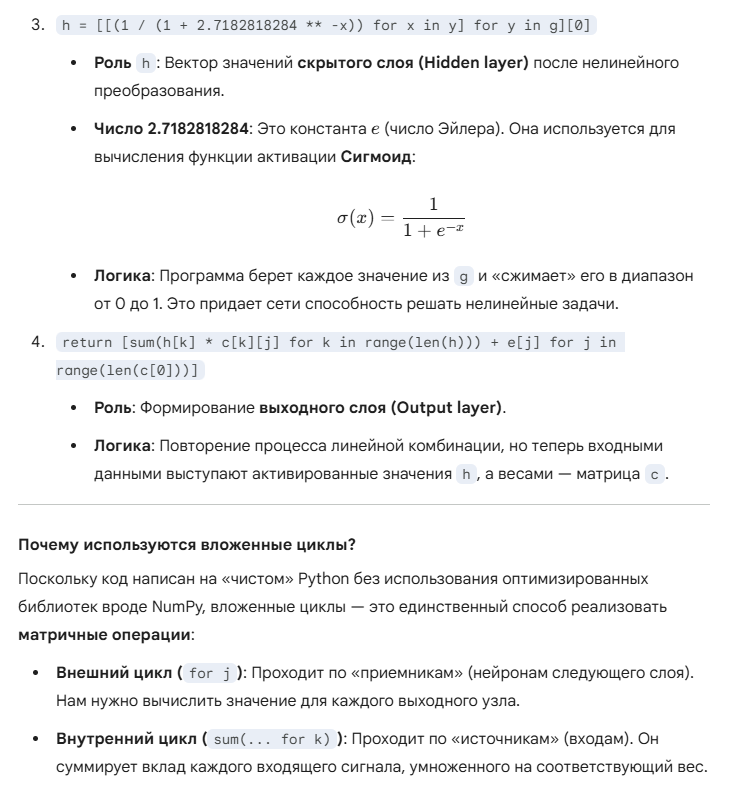
\includegraphics[width=17cm]{z1/2-2.png}
	\caption{ч.2}
\end{figure}
\newpage
\begin{figure}[H]
	\centering
	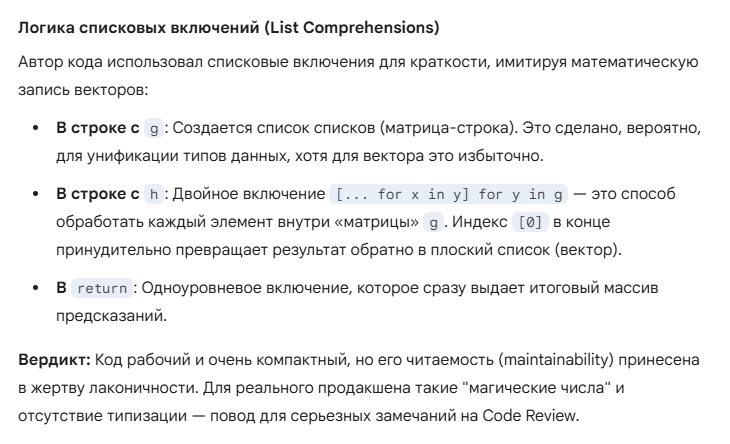
\includegraphics[width=17cm]{z1/2-3.png}
	\caption{ч.3}
\end{figure}
\noindent
\indent Анализ: Ответ глубокий, но отсутствовала таблица соответствия. Попросил дополнить таблицей. \\
\newline
\indent Корректирующий промпт:
\textit{«Отлично. Теперь представь расшифровку переменных в виде таблицы: старое имя → осмысленное имя (например, x → input\_batch) и краткое описание. В ответ выдай только таблицу.»}
\newpage
Ответ модели:
\begin{figure}[H]
	\centering
	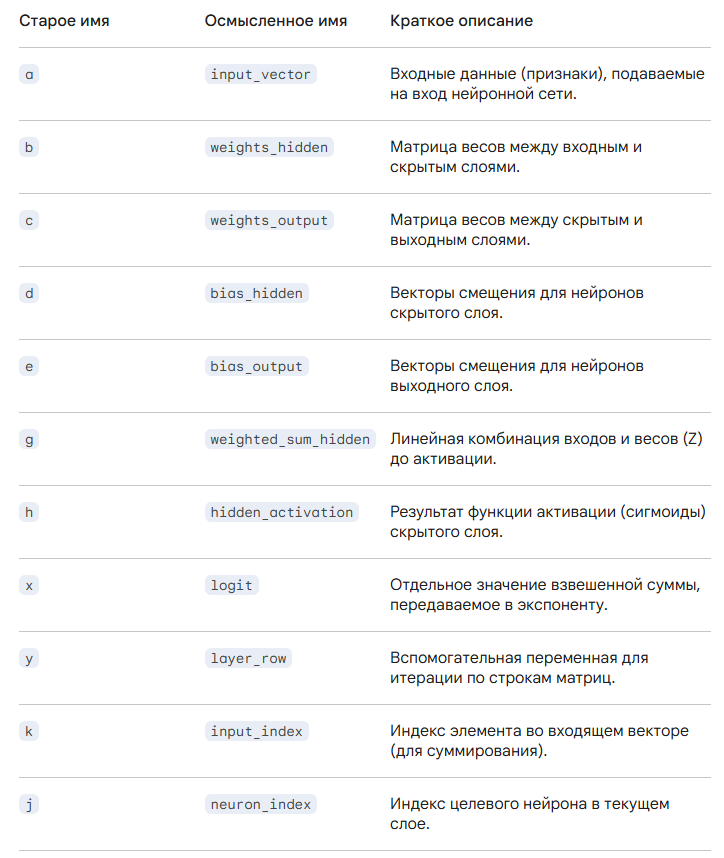
\includegraphics[width=17cm]{z1/3-1.png}
	\caption{Таблица}
\end{figure}
\newpage
\noindent
\textbf{Этап 3. Структурная абстракция и визуализация логики} \\
\indent Промпт:
\textit{«Сгенерируй псевдокод этого алгоритма на русском языке, опустив синтаксический шум Python. Затем создай описание блок-схемы в формате Mermaid (код, который можно вставить в Markdown).»}\\
\newline
\noindent
Ответ модели (псевдокод): \\
АЛГОРИТМ: Прямой проход двухслойной нейронной сети \\
ВХОД: Вектор\_Входа, Веса\_Скрытого\_Слоя, Веса\_Выхода, \\ \indent Смещение\_Скрытого\_Слоя, Смещение\_Выхода \\
\newline
\noindent
ШАГ 1: Вычисление скрытого слоя (линейная часть)
   Для каждого нейрона в скрытом слое:
      Сумма = 0
      Для каждого элемента во Векторе\_Входа:
         Сумма = Сумма + (Входной\_Элемент * Соответствующий\_Вес\_Скрытого\_Слоя)
      Результат\_Скрытый{[}нейрон{]} = Сумма + Смещение\_Скрытого\_Слоя{[}нейрон{]}\\
\newline
\noindent
ШАГ 2: Активация скрытого слоя (нелинейность)
   Для каждого значения в Результат\_Скрытый:
      Активация{[}нейрон{]} = 1 / (1 + Экспонента(-Значение))  // Функция Сигмоида \\
\newline
\noindent
ШАГ 3: Вычисление выходного слоя
   Для каждого нейрона в выходном слое:
      Сумма = 0
      Для каждого элемента в Активация:
         Сумма = Сумма + (Активированный\_Элемент * Соответствующий\_Вес\_Выхода)
      Прогноз{[}нейрон{]} = Сумма + Смещение\_Выхода{[}нейрон{]} \\
\newline
\noindent
ВЫХОД: Прогноз
\newpage
Блок-схема в формате Mermaid:
\begin{figure}[H]
	\centering
	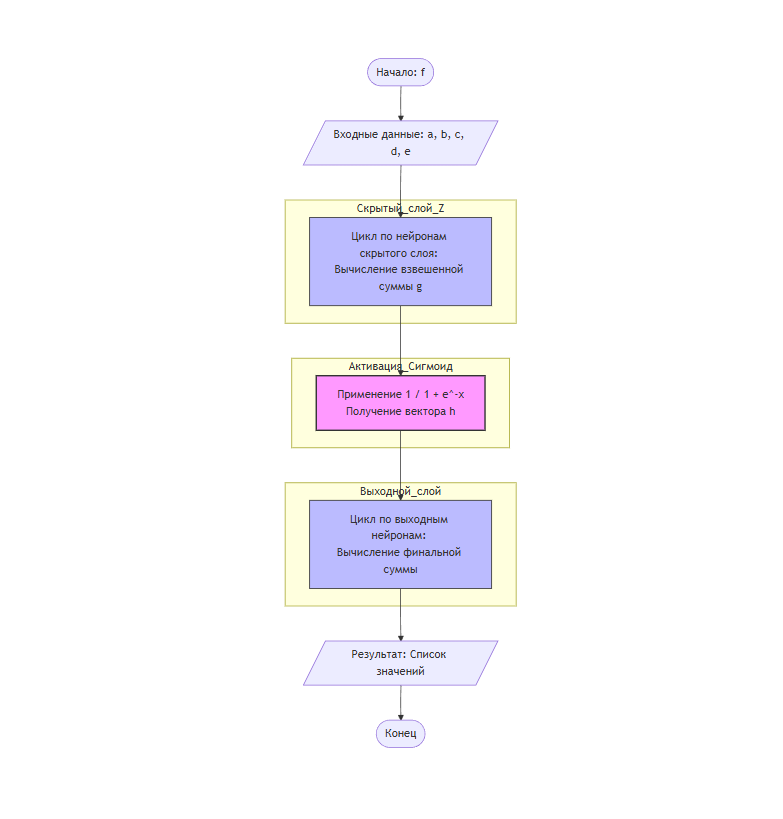
\includegraphics[width=17cm]{z1/4-1.png}
	\caption{Блок-схема}
\end{figure}
Анализ: Псевдокод и диаграмма корректно отражают логику. Вложенные циклы заменены абстракцией матричного умножения, что упрощает понимание.
\newpage
\noindent
\textbf{Этап 4. Верификация через гипотетическое тестирование (Socratic Method)} \\
Промпт:
\textit{«Ответь на вопросы, ссылаясь на конкретные строки исходного кода:
1. Что произойдёт, если на вход подать пустой список x = {[}{]}?
2. Как поведёт себя код, если размерности <<b>> и <<a>> не согласованы (например, число столбцов <<a>> не равно числу строк <<b>>)?
3. Есть ли в коде потенциальная утечка памяти или неэффективность?»} \\
\newline
\noindent
Ответ модели:
\begin{figure}[H]
	\centering
	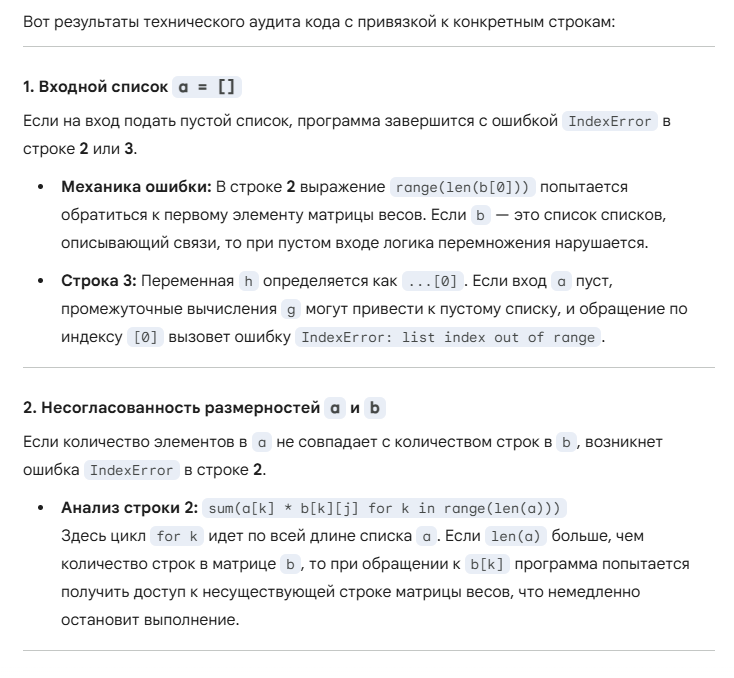
\includegraphics[width=15cm]{z1/5-1.png}
	\caption{ч.1}
\end{figure}
\newpage
\begin{figure}[H]
	\centering
	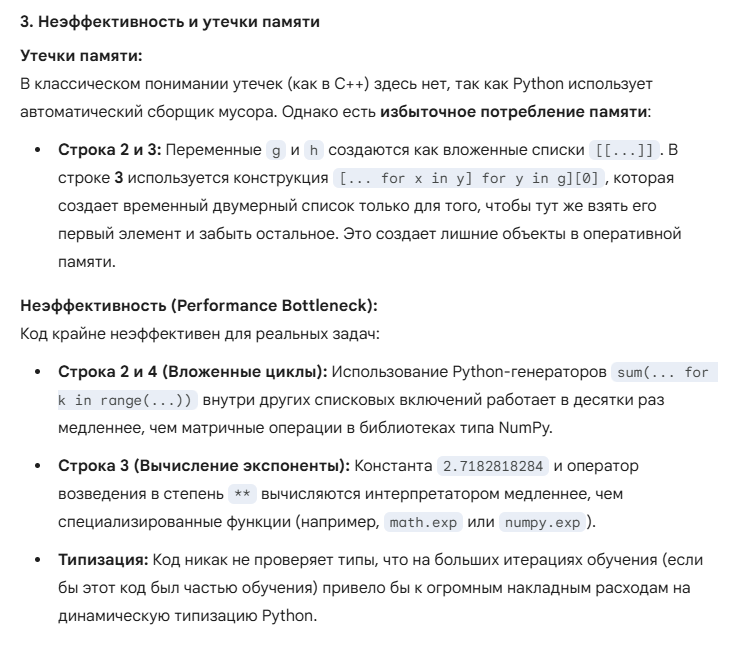
\includegraphics[width=17cm]{z1/5-2.png}
	\caption{ч.2}
\end{figure}
Анализ: Модель корректно просимулировала выполнение, указала на отсутствие валидации входных данных и на не эфективное использование памяти. Моя корректировка не потребовалась.
\newpage
\noindent
\textbf{Этап 5. Синтез итоговой документации} \\
\indent Промпт:
\textit{«Объедини всю информацию из диалога в единый структурированный документ, который включает:
Исходный «плохой» код,
Краткое резюме назначения,
Таблицу расшифровки переменных,
Пошаговое описание алгоритма на русском,
Выявленные ограничения и потенциальные проблемы.
Документ должен выглядеть как профессиональная документация.»} \\
\newline
\noindent
Модель выдала итоговый документ (см. раздел 1.4).
\subsection{Артефакты}
Исходный «грязный» код:
\lstinputlisting[language=Python]{z1/0.py}
\newpage
Итоговое структурированное описание алгоритма от модели:
\begin{figure}[H]
	\centering
	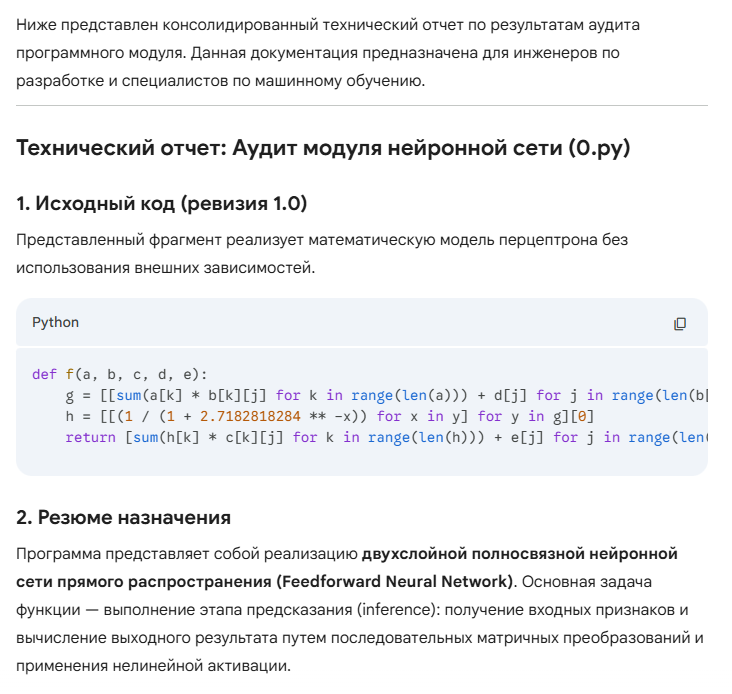
\includegraphics[width=17cm]{z1/6-1.png}
	\caption{ч.1}
\end{figure}
\newpage
\begin{figure}[H]
	\centering
	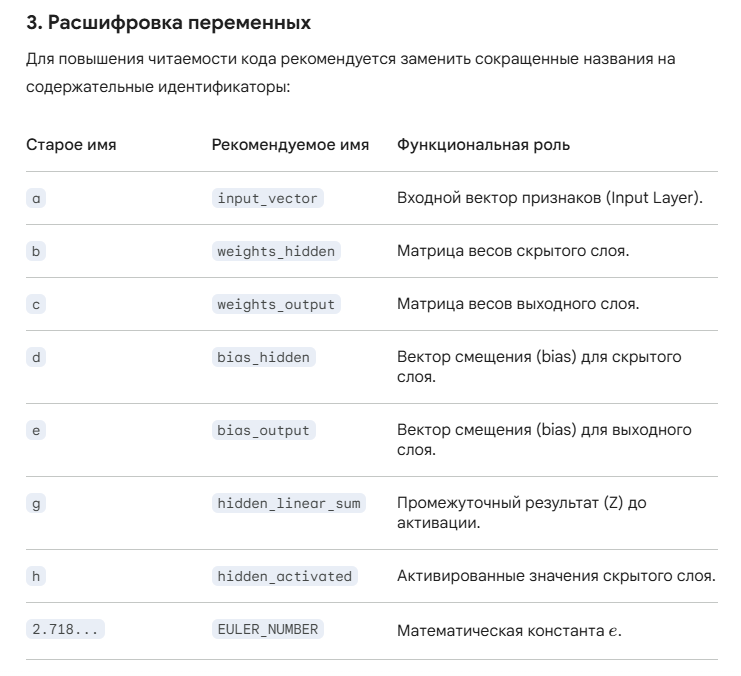
\includegraphics[width=17cm]{z1/6-2.png}
	\caption{ч.2}
\end{figure}
\newpage
\begin{figure}[H]
	\centering
	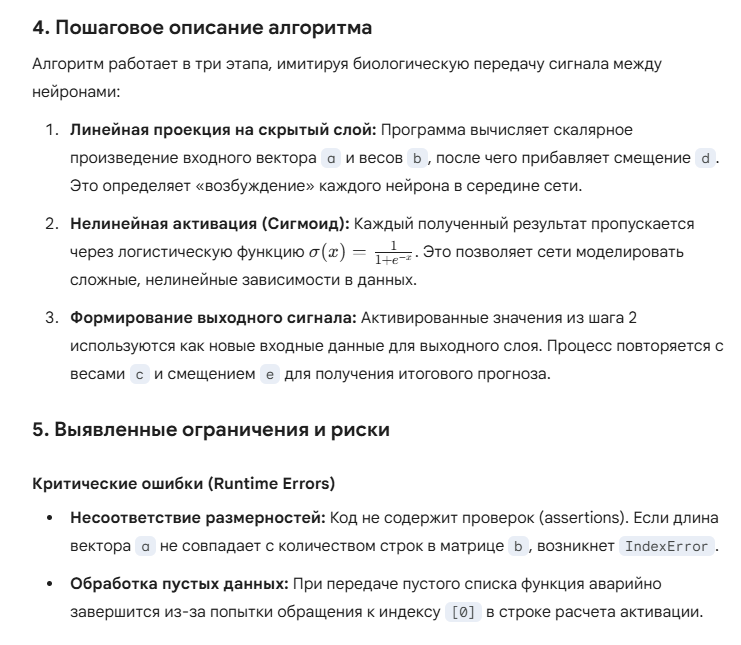
\includegraphics[width=17cm]{z1/6-3.png}
	\caption{ч.3}
\end{figure}
\newpage
\begin{figure}[H]
	\centering
	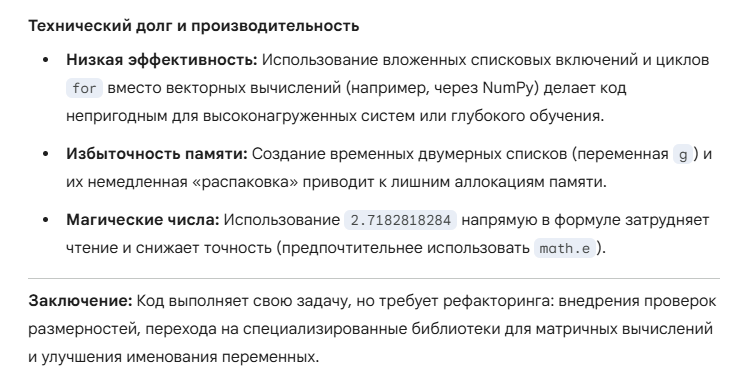
\includegraphics[width=17cm]{z1/6-4.png}
	\caption{ч.4}
\end{figure}
\subsection{Сравнение моделей (Benchmarking)}
Для ознокомления тот же чат но с моделью (b): \\
https://chat.deepseek.com/share/43ysvnxaa1wa159vzf
\begin{table}[h!]
	\centering
	\begin{tabular}{|l|p{5cm}|p{5cm}|}
		\hline
		\textbf{Критерий} & \textbf{модель (a)} & \textbf{модель (b)} \\
		\hline
		Глубина деобфускации & 5 & 5 \\
		\hline
		Полнота описания алгоритма & 4 & 6 \\
		\hline
		Корректность визуализации & 4 & 3 \\
		\hline
		Способность к самокоррекции & 4 & 5 \\
		\hline
		\textbf{Итог} & 4.25 & 4.75\\
		\hline
	\end{tabular}
\end{table} \\
Итог: Обе модели в целом справились с задачей. Модель (b) дала более структурированный и полный ответ (включая псевдокод и детальные ограничения), но хуже сгенерировала Mermaid. Модель (a) в этом плане более универсальная модель.
\newpage
\subsection{Вывод}
\noindent
Наиболее эффективными техниками промпт-инжиниринга оказались:
\begin{itemize}
	\item Ролевое моделирование (задание роли «небрежного разработчика» для генерации кода и «Senior-аудитора» для анализа) – позволило получить нужный стиль и глубину проверки.
	\item Chain of Density (последовательное уточнение: сначала общий анализ, затем таблица переменных) – улучшило детализацию.
	\item Верификация через гипотетическое тестирование (Socratic questioning) – выявило скрытые недостатки (обработка пустого входа, отсутствие проверок размерностей).
	\item Визуализация логики (Mermaid) – упростила понимание блок-схемы.
\end{itemize}
Без итеративного подхода модель могла выдать только поверхностное описание. Применение контрольной модели подтвердило, что финальный промпт является достаточно универсальным, хотя незначительные различия в выводе показывают необходимость адаптации под конкретную LLM.
